\documentclass[a4paper, 12pt, draft]{article}
\usepackage{graphicx}
\usepackage[utf8]{inputenc}
\usepackage{multirow}
%\usepackage{times}
\usepackage{listings}
\usepackage{supertabular}
\usepackage{cite}
\usepackage{amsthm}
\usepackage{tikz}

\newcommand{\jcode}[1]{\textnormal{\texttt{#1}}}
\newcommand{\pcode}[1]{\textnormal{\texttt{#1}}}
\newcommand{\pmodule}[1]{\textnormal{\texttt{#1}}}
\newcommand{\rdfterm}[1]{\textnormal{\textsf{#1}}}

\include{helpers}
\usepackage[pdftex,linktocpage]{hyperref}

\begin{document}
\title{Prefetching SPARQL query cacher}
\author{Kjetil Kjernsmo}
%\institute{Department of Informatics,
%Postboks 1080 Blindern,
%0316 Oslo, Norway}

%\email{kjekje@ifi.uio.no}

\maketitle

\section{Introduction}

This chapter describes an effort to create a proxy that can cache the
results of not only SPARQL queries, but also the results of individual
triple patterns. It will asynchronously analyse executed queries, and
may prefetch the results of certain triple patterns into the cache.

The system is in the convergence of the directions described in this
dissertation: It should relieve the remote endpoint of some of the
burden to evaluated the query and it should add to the robustness of the
open Web SPARQL infrastructure. It uses hypermedia to answer individual
triple patterns, based on Triple Pattern Fragments  \cite{ldf1}. The
system can only answer triple patterns, but other than that, supports
SPARQL 1.1 in its entirety. This was made possible to develop quickly
by the efforts put into the query planning in the Attean framework
described in Section~\ref{sec:conpush}. Caching based on RFC7234
\cite{rfc7234} was shown to be of possible use in the survey I
conducted. Finally, it was planned to be evaluated using
Design of Experiments.

Unfortunately, the system has as of this writing insufficient
performance for an evaluation to be meaningful. Nevertheless, it
points out some interesting lessons with varying degrees of
certainty. This chapter will detail the system, show its design and
features and discuss its failures.

\begin{figure}
\begin{center}
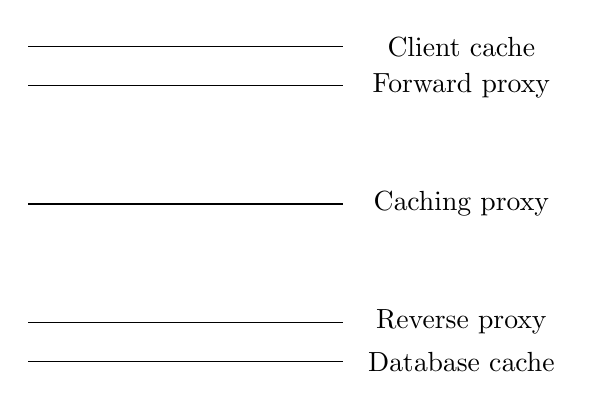
\begin{tikzpicture}
\draw (0,0) --(4,0);
\node at (5.5,0) { Database cache };
\draw (0,0.5) --(4,0.5);
\node at (5.5,0.5) { Reverse proxy };
\draw (0,2) --(4,2);
\node at (5.5,2) { Caching proxy };
\draw (0,3.5) --(4,3.5);
\node at (5.5,3.5) { Forward proxy };
\draw (0,4) --(4,4);
\node at (5.5,4) { Client cache };
\end{tikzpicture}
\caption{The possible positions of a cache. A cache may reside at both
  the server side or client side, or any of the intermediate
  proxies. The database proxy and reverse proxy is typically
  controlled by the data provider.}
\end{center}
\end{figure}


\bibliography{management,dataprofiles,federation,dynamicity,hypermedia,specs,webarch,practical,semweb,caching,critisism,data,philosophy,benchmarks,rfc,programming,egne}
\bibliographystyle{plain}

\end{document}
